\subsubsection{k-Nearest Neighbors (KNN) Analysis}
\label{subsubsec:discussion-knn}

This section interprets the results of the KNN algorithm, discussing its performance and implications.

The KNN algorithm was evaluated using several performance metrics, including accuracy, precision, and recall and the f1 score.

\subsubsection*{General Performance Analysis}
As seen in Tables 1 and 2, the general performance of the KNN algorithm was excellent across both datasets,
achieving accuracy scores above 92\% and F1 scores above 92.5\% on all top ten configurations.

\subsubsection{Mushroom Dataset Performance}

\begin{description}
    \item[\textbf{Best Configuration:}]\leavevmode
        \begin{itemize}
            \item $k = 3, 5,$ or $7$ with Manhattan Distance (all performed equally well)
            \item Shepard's Work Voting scheme
            \item Equal Weighting
            \item \textbf{Results:} 95.1\% accuracy and 95.2\% F1 score
        \end{itemize}
    
    \item[\textbf{Performance Range:}]\leavevmode
        \begin{itemize}
            \item Accuracy: 92.6\% $--$ 95.1\%
            \item F1 Score: 92.7\% $--$ 95.2\%
        \end{itemize}
\end{description}

\subsubsection*{Observations}
Manhattan Distance consistently performed well across all configurations, with all top ten configurations using this distance metric.
The combination of Manhattan Distance and Shepard's Work Vote with a higher value of k was particularly effective. 
The higher performance of a larger k value suggests that the algorithm benefits from considering multiple neighbors when making predictions, perhaps
due to the dataset's inherent complexity and noise present in the data. The equal weighting scheme also performed excellently,
indicating that the dataset contains relatively a uniform
distribution of meaningful data points.
The F1 scores achieved across all configurations were consistently high, indicating a good balance between precision and recall.

\begin{figure}
    \centering
    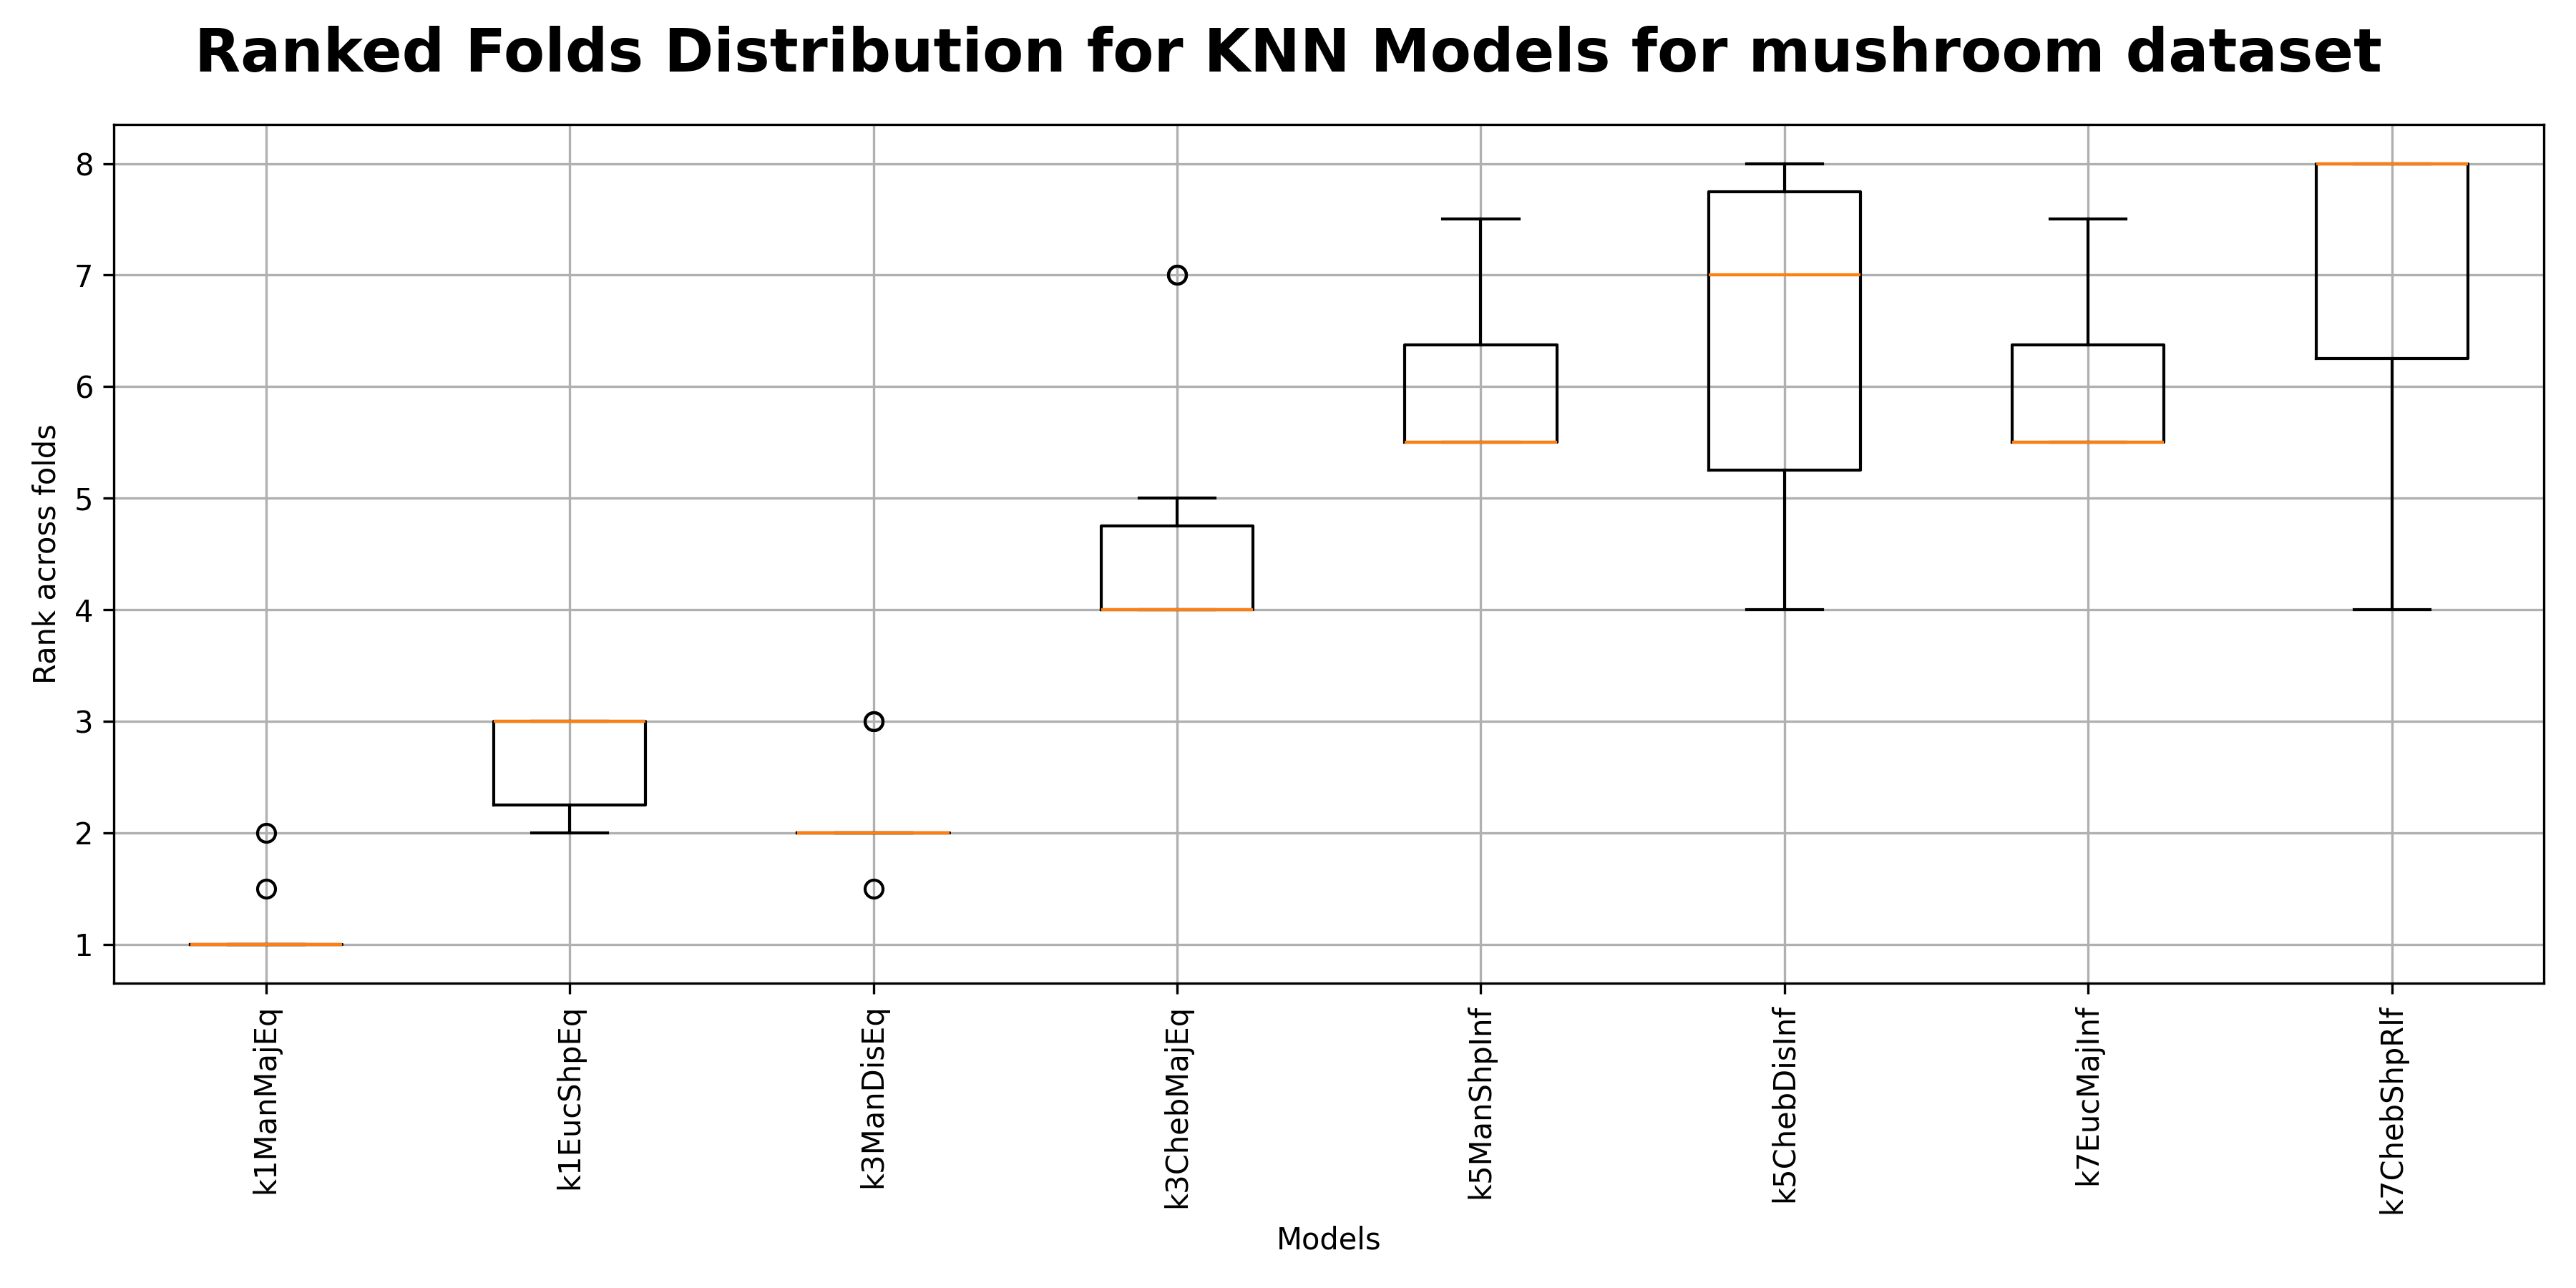
\includegraphics[width=0.9\textwidth]{figures/ranked_folds_KNN_mushroom.png}
    \caption{KNN Ranked Folds for Mushroom Dataset}
    \label{fig:ranked_folds_KNN_mushroom}
\end{figure}

The above figure shows the ranked folds for the k-NN algorithm on the mushroom dataset.
The figure illustrates the variation in performance across different KNN models, with some models performing 
better than others. It's evident a lower value of k (1 or 3) tends to perform better than higher values of k (5 or 7)
in combination with the other parameters. 
Interestingly, for each KNN model the performance across the 10 folds is identical.

\subsubsection{Hepatitis Dataset Performance}

\begin{description}
    \item[\textbf{Best Configuration:}]\leavevmode
        \begin{itemize}
            \item $k = 1$ with Euclidean Distance
            \item Shepard's Work Vote
            \item ReliefF Weighting
            \item \textbf{Results:} 95.5\% accuracy and 97.2\% F1 score
        \end{itemize}
    
    \item[\textbf{Performance Range:}]\leavevmode
        \begin{itemize}
            \item Accuracy: 94.8\% $--$ 95.5\%
            \item F1 Score: 96.7\% $--$ 97.2\%
        \end{itemize}
    
    \item[\textbf{Key Observations:}]\leavevmode
        \begin{itemize}
            \item Euclidean Distance performed best, particularly with ReliefF weighting.
            \item k = 1 configurations dominated the top results.
            \item All voting schemes performed similarly when other parameters were optimized.
        \end{itemize}
\end{description}

\subsubsection*{Observations}
The hepatitis dataset achieved its best performance with a k value of 1, indicating that the algorithm benefits from
more localized decisions when making predictions when using this dataset.
The Euclidean Distance metric performed best, particularly when combined with ReliefF weighting. This suggests that the dataset's features
have varying degrees of importance, and ReliefF weighting helps capture these distinctions effectively.
As also seen in the mushroom dataset, the F1 scores achieved across all configurations were consistently high,
indicating a good balance between precision and recall.


\begin{figure}
    \centering
    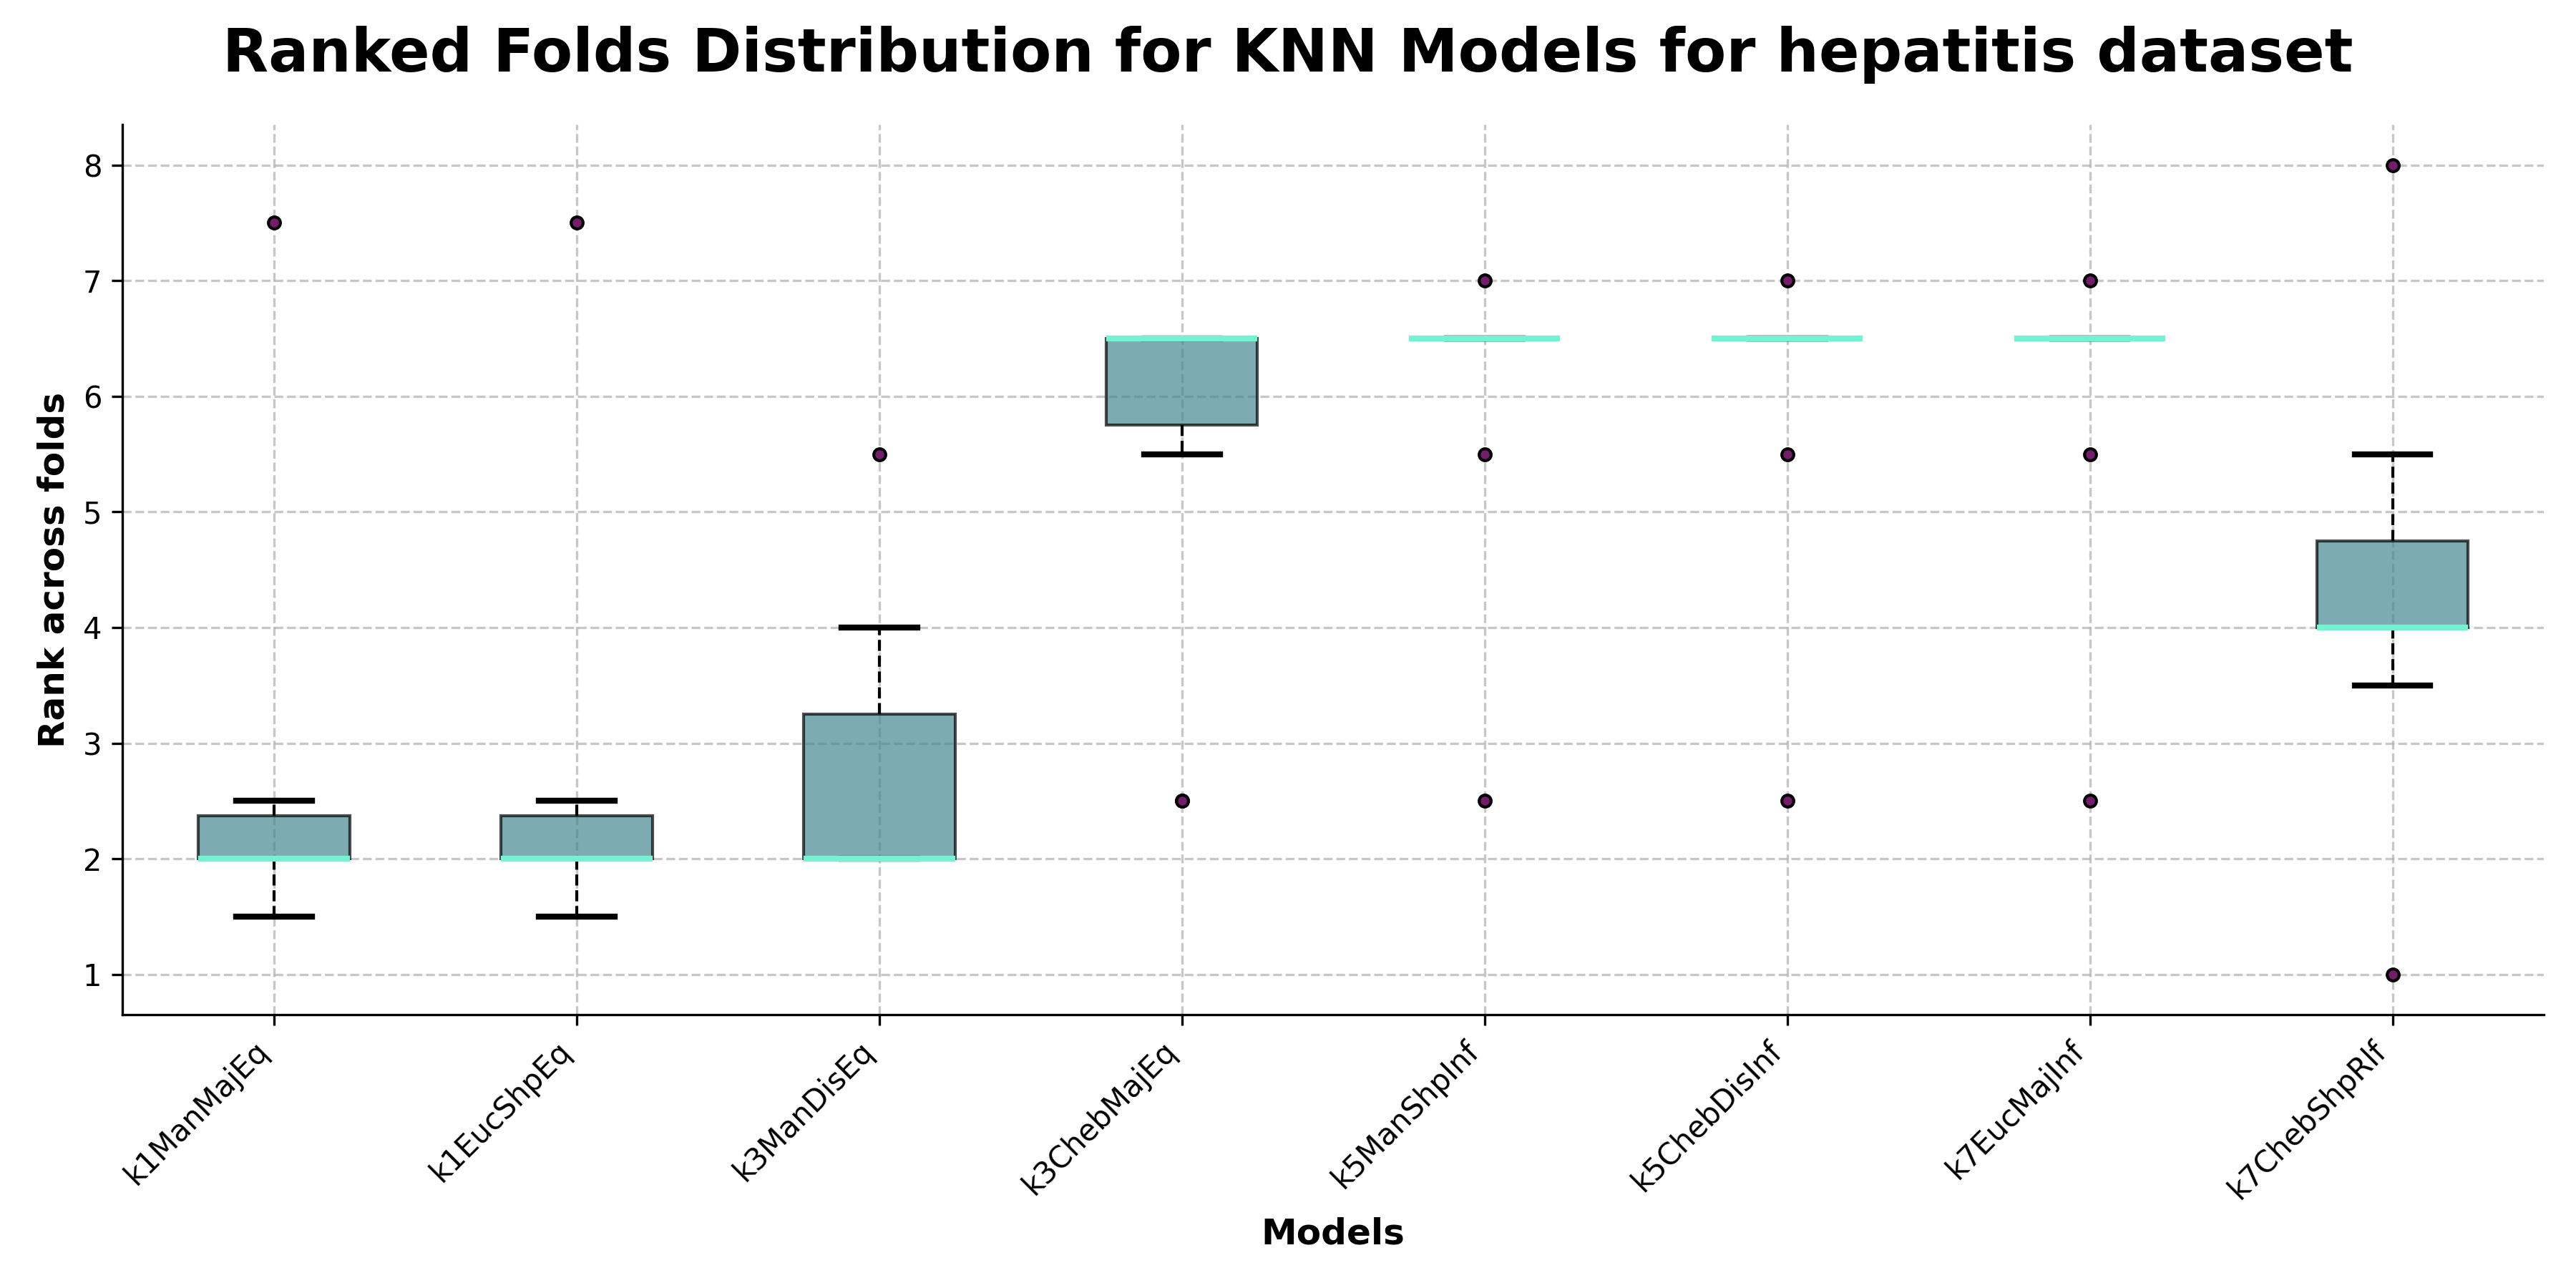
\includegraphics[width=0.9\textwidth]{figures/ranked_folds_KNN_hepatitis.png}
    \caption{KNN Ranked Folds for Hepatitis Dataset}
    \label{fig:ranked_folds_KNN_hepatitis}
\end{figure}

The above figure shows the ranked folds for the k-NN algorithm on the mushroom dataset.
The figure illustrates the variation in performance across different KNN models, with some models outperforming others.
Unlike the mushroom dataset, the hepatitis dataset shows variation in performance in each model per fold.
A number of the models showed consistent mean performance but also contained some outliers that performed significantly better or worse
than the mean.


\subsubsection{Overall Comparison}
While both datasets achieved high performance, the hepatitis dataset outperformed the mushroom dataset in terms of accuracy and F1 score.
This difference may be due to the hepatitis dataset's smaller size and more distinct class separations,
making it easier for the KNN algorithm to make accurate predictions. These distinct class separations may also explain why the k = 1 configuration
performed best on the hepatitis dataset, as the algorithm can make more precise decisions with fewer neighbors.

\subsection*{K-Nearest Neighbour (KNN) Statistical Analysis}
Below are the Nemenyi test results for the KNN models on the hepatitis and mushroom datasets respectively.

For the below analysis of both the KNN model, values closer to 1 indicate no significant difference between models,
whereas values closer to 0 indicate a significant difference.

The diagonal values (top left to bottom right) are always 1 and report no significant difference
as they represent the comparison of a model with itself.

To determine statistical significance, we use a confidence level of 0.95 (95\% confidence interval) for the Nemenyi test.
Therefore, any values greater than 0.05 indicate that the models are not significantly different from each other.

\begin{figure}[!ht]
    \centering
    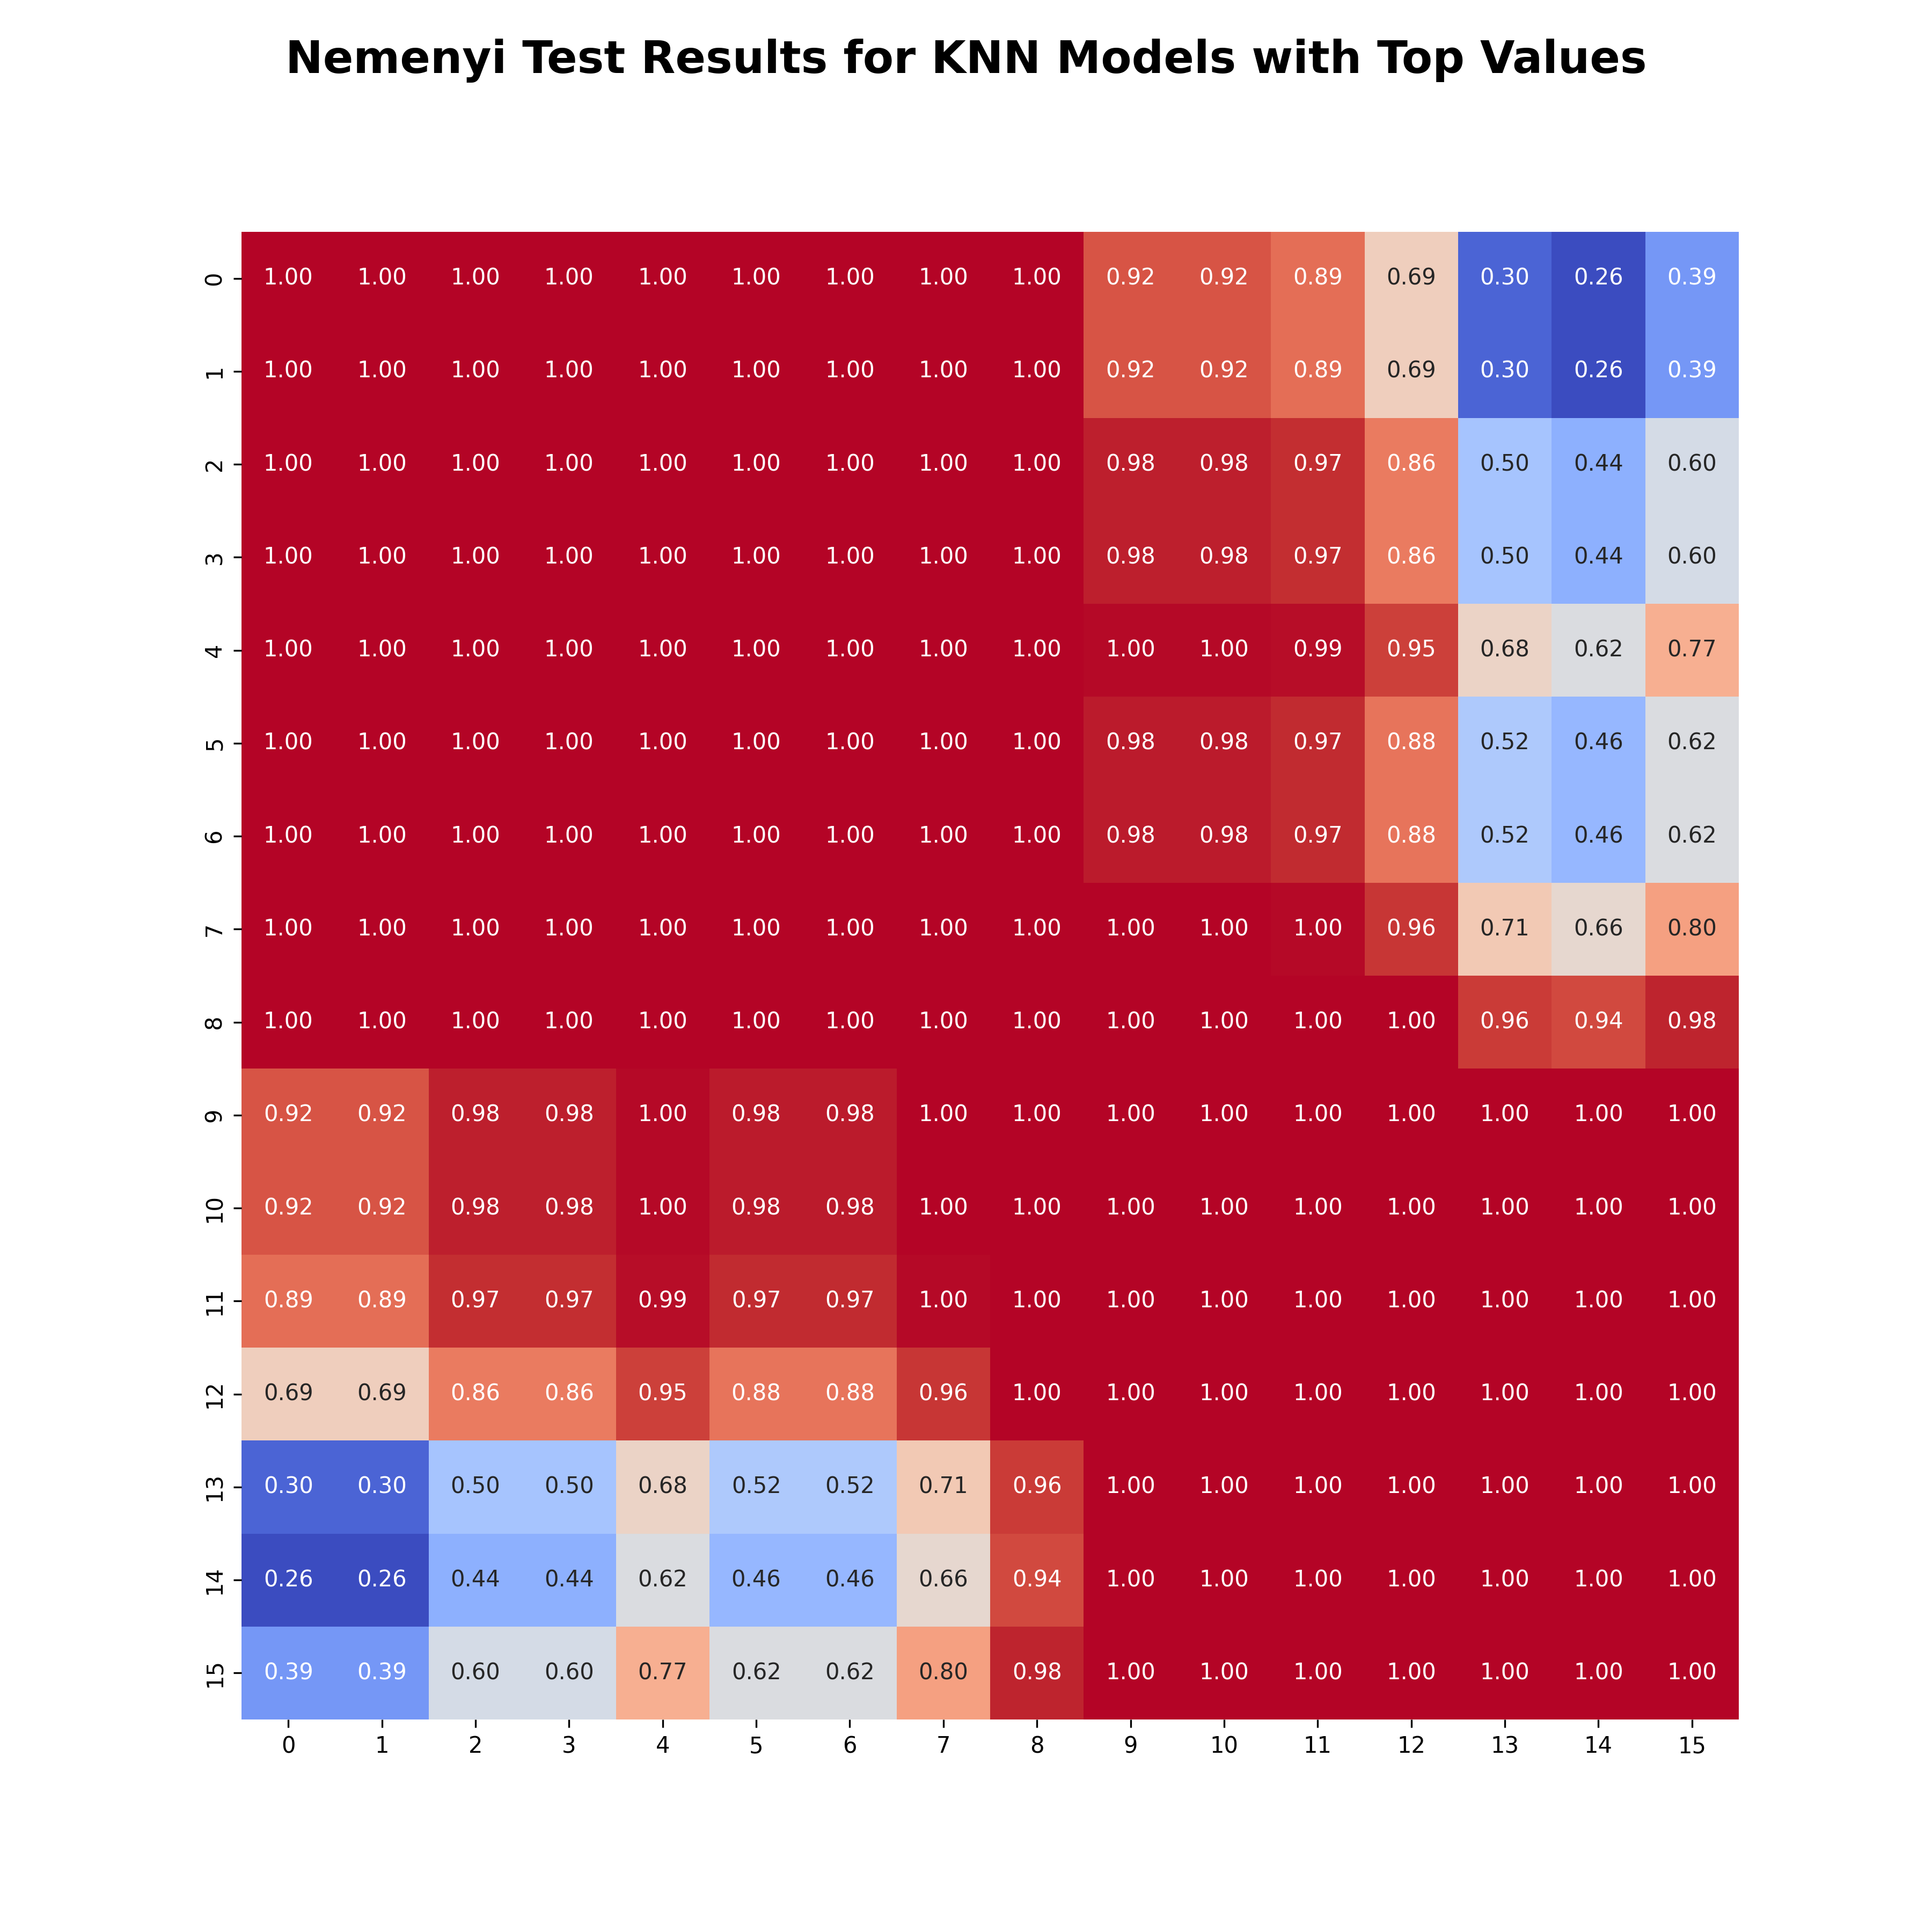
\includegraphics[width=0.8\textwidth]{figures/nemenyi_test_results_KNN_hepatitis.png}
    \caption{Nemenyi test results for KNN models on the hepatitis dataset}
\label{fig:nemenyi_test_results_KNN_hepatitis}
\end{figure}

\begin{figure}[!ht]
    \centering
    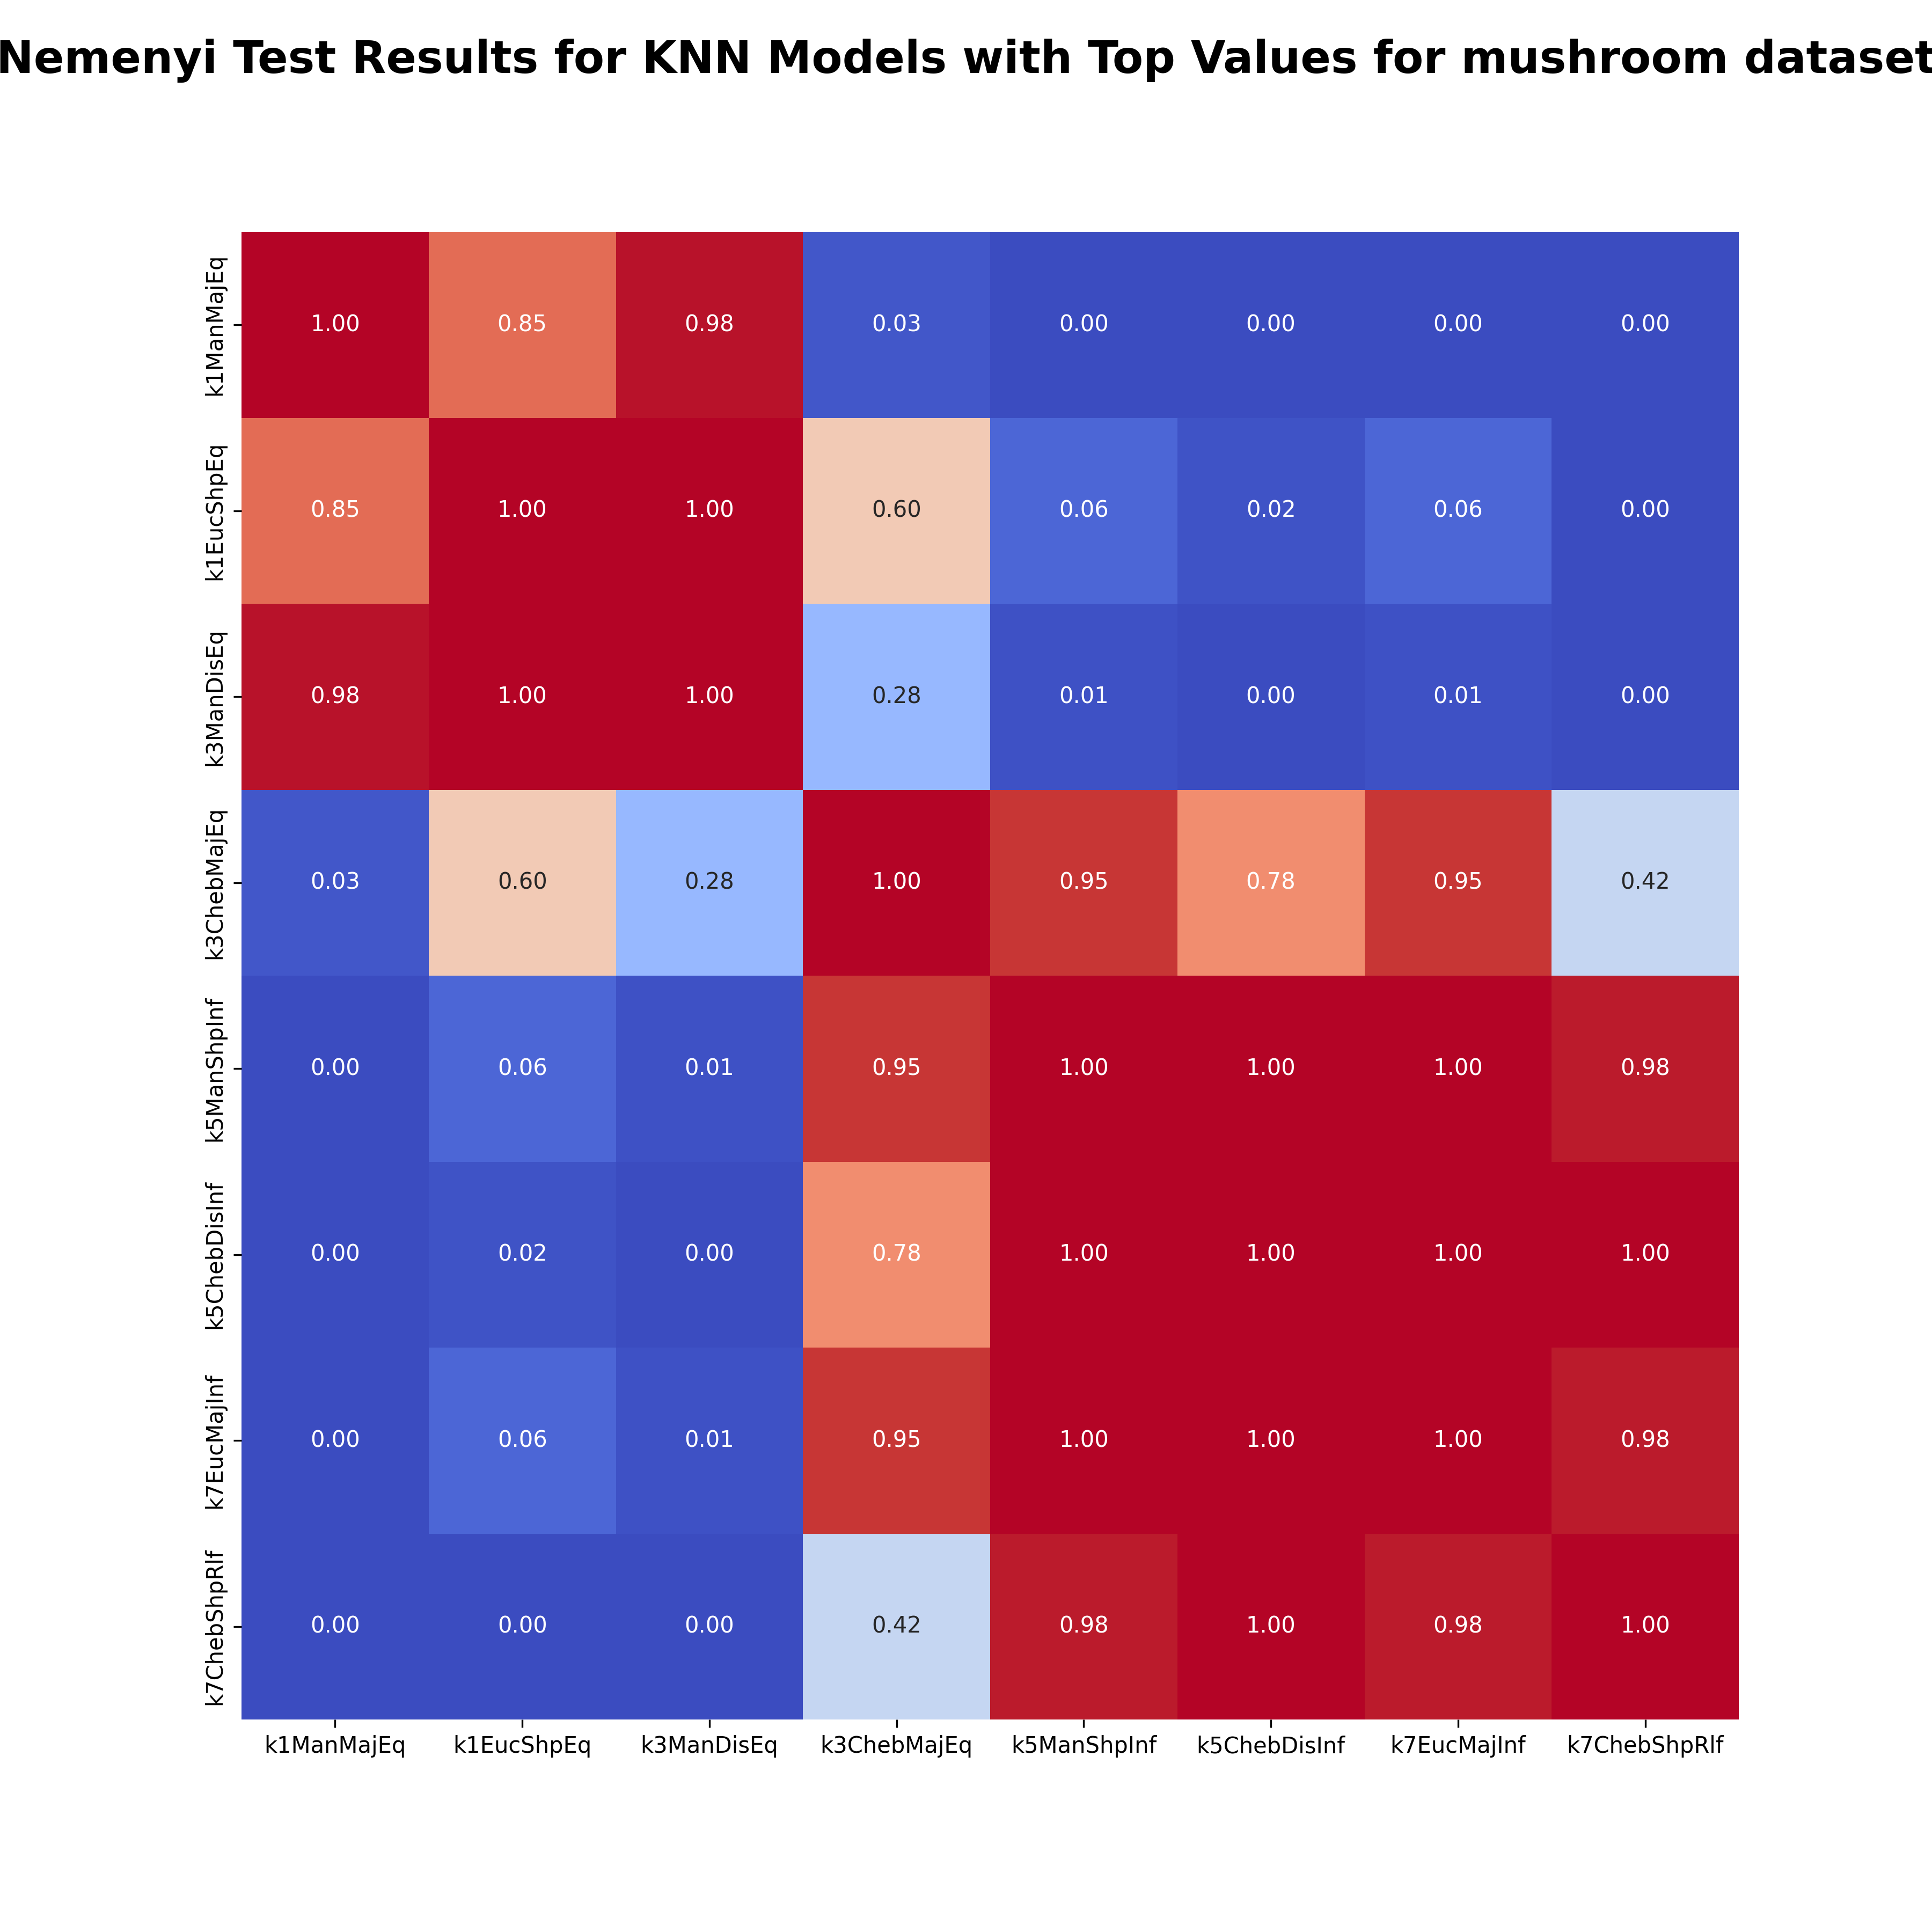
\includegraphics[width=0.8\textwidth]{figures/nemenyi_test_results_KNN_mushroom.png}
    \caption{Nemenyi test results for KNN models on the mushroom dataset}
\label{fig:nemenyi_test_results_KNN_mushroom}
\end{figure}

The Nemenyi test results for the KNN models on the hepatitis dataset reveal two statistically distinct
groups of model configurations. The first group consists of k = 1 configurations
(with Manhattan and Euclidean distance) and k=3 with Manhattan distance, which all perform similarly to each other (p=1.00).
The second group includes configurations with higher k values (3,5,7) using various distance metrics,
which also perform similarly within their group (p=1.00) but significantly differently from the first
group (some comparisons yield p=0.04, below the 0.05 threshold). This clear separation suggests that the choice of k-value
has a more substantial impact on model performance than the choice of distance metric, with k=1 configurations behaving distinctly from higher k-values.

The Nemenyi test results for the KNN models on the mushroom dataset reveal two main groups of model configurations.
The first group consists of k=1 configurations and k=3 with Manhattan distance, which perform similarly
(p=0.85 $-$ 1.00), though with some variation within the group. The second group includes configurations
from k5ManShpInf through k7ChebShpRtf, which show high similarity within their group (p=0.95 $-$ 1.00).
Some of these groups perform significantly differently from each other, given the p-values fall below the 0.05 threshold.

We can deduce that the k-value has a substantial impact on model performance on both datasets. 

\subsubsection*{Parameter Analysis}

\begin{figure}[!ht]
    \centering
    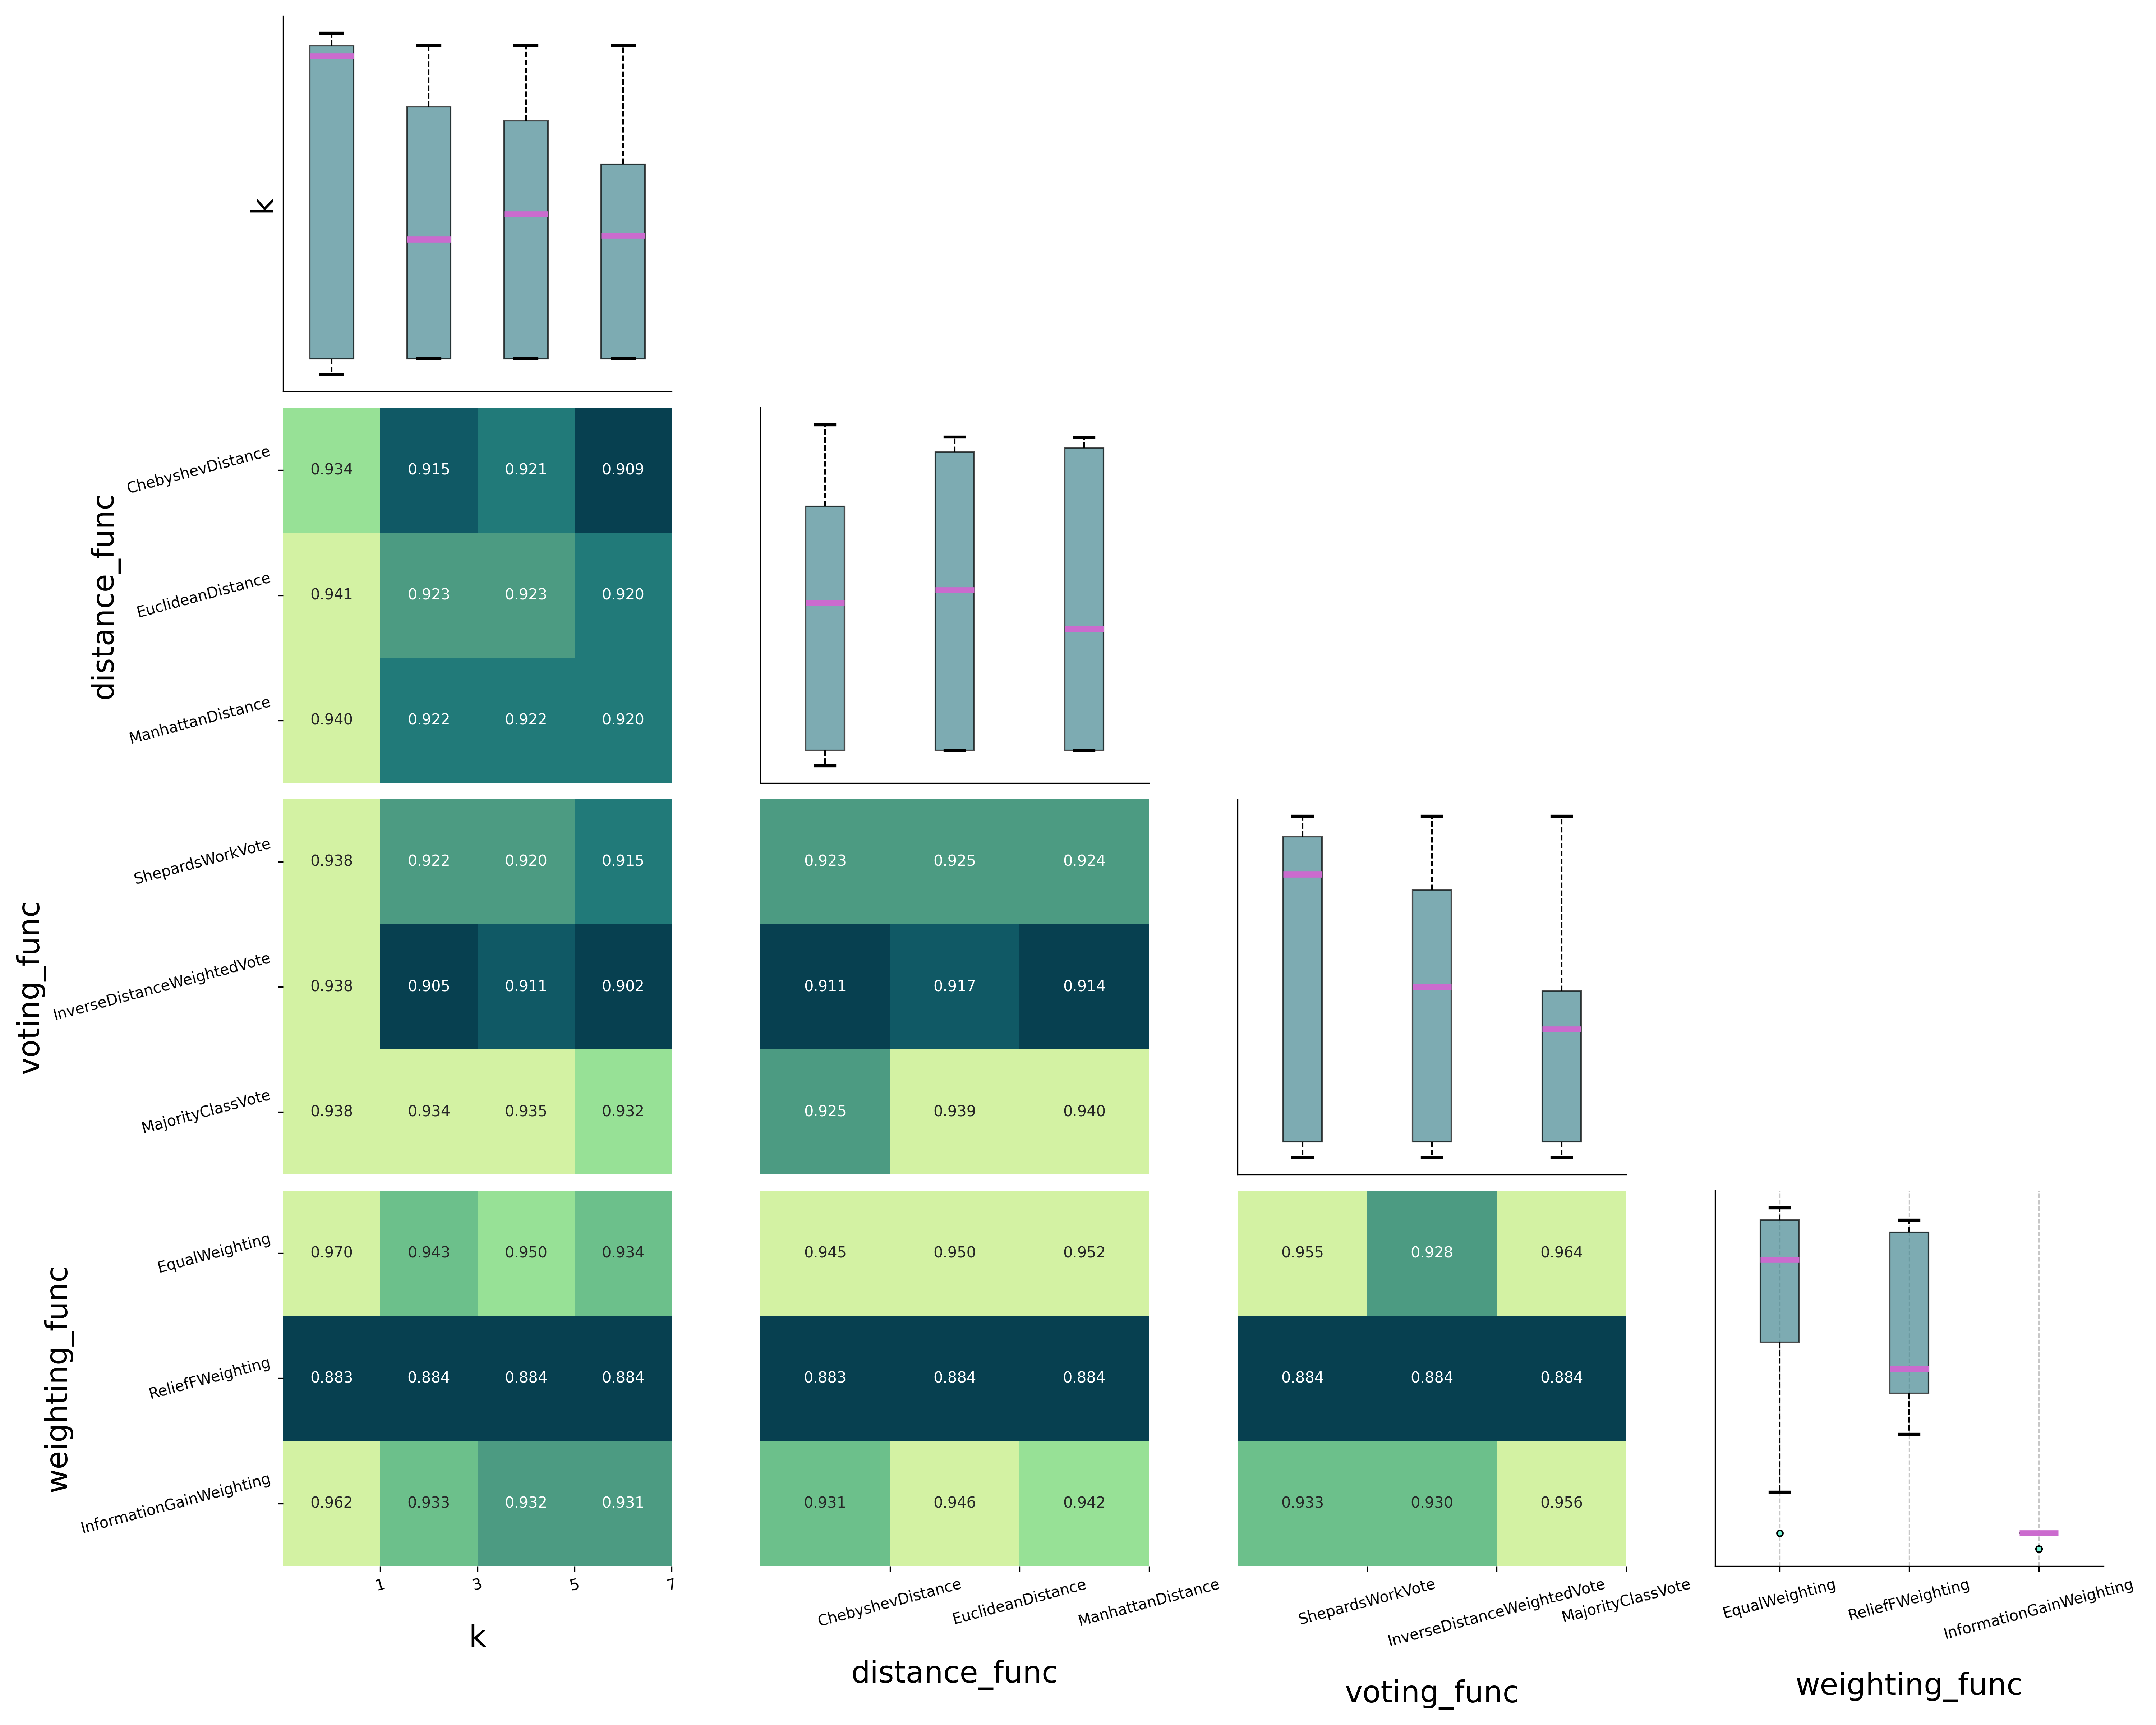
\includegraphics[width=0.8\textwidth]{figures/interaction_effects_KNN_hepatitis.png}
    \caption{Interaction effects for KNN models on the hepatitis dataset}
\label{fig:interaction_effects_KNN_hepatitis}
\end{figure}

To further understand the impact of the parameters on the performance of the KNN algorithm,
we analyzed the impact of the hyperparameters on the performance of the KNN algorithm, both independently and in combination.

We can see from \autoref{fig:interaction_effects_KNN_hepatitis} that each parameter plays a significant role in the performance of the KNN algorithm.
We also see some notable interactions between parameters, such as majority class voting performing better when combined with low k values and the Manhattan distance metric.
We also see that Inverse Distance Weighting performs poorly in all cases except with k=1, where it there is difference at all (since voting scheme has no impact when k=1).
